\documentclass[11pt]{article}
\usepackage[final]{acl2023}
\usepackage{times}
\usepackage{latexsym}
\usepackage{amsmath,amssymb,booktabs,graphicx}
\usepackage[T1]{fontenc}
\usepackage[utf8]{inputenc}
\usepackage{microtype}
\title{Talk Like a Structured Graph: Augmenting Text Encodings with Structural Statistics}
\author{
  Inbal Moryles\\
  \footnotesize\texttt{github.com/iinbal}
  \And
  Gal Barak\\
  \footnotesize\texttt{github.com/GalBrk}
  \And
  Nitzan Zacharia\\
  \footnotesize\texttt{github.com/NitzanZacharia}
}
\date{}
\begin{document}
\maketitle
\begin{abstract}
Can verbalized graph statistics improve language-model graph reasoning beyond supplying answers or changing response procedures? We prepend degree, clustering, and random-walk return probabilities to incident-text graph encodings. In paired tests on 40-node graphs, Qwen3-1.7B and Qwen3-4B answer six GraphQA questions with plain and thinking prompts. Degree helps most where it states the answer, but harms a model that already counts neighbors reliably. A smaller clustering effect replicates on fresh graphs but varies with node position. Thinking helps some tasks yet often exhausts the response budget on edge counts. We audit primer-only shortcuts and report truncation separately: gains depend on disclosed information, reading procedure, and output budget.
\end{abstract}

\section{Introduction}
\label{sec:intro}
\textbf{Research question.} When a black-box language model reads a textual graph, do explicit structural statistics improve execution of graph queries, and can their effect be distinguished from answer leakage and changes in how the graph is read? This question matters because a graph encoding may contain every necessary edge while leaving the model unable to execute a simple count or maintain consistency between related answers.

GraphQA reports that graph representation, task, and topology jointly affect language-model performance \citep{fatemi2023talklikeagraph}; NLGraph likewise documents limits on solving graph problems described in text \citep{wang2023nlgraph}. Graph Transformers can consume structural or positional information numerically, including random-walk structural encodings (RWSE) \citep{rampasek2022recipe,dwivedi2022graph}. Translating these compact numerical features into a long, node-indexed English preamble is an uncertain interface: the model must locate the right node, interpret rounded statistics, and still read the original edges. Results for a graph Transformer do not establish that the same information will help a frozen LLM.

We distinguish three mechanisms: a feature can \emph{state} an answer, change its extraction \emph{procedure}, or offer \emph{side information} for graph reading. Our paired study tests gains and failures with a graph-blind shortcut audit, length control, task-sensitive scores, and truncation as a third outcome.

\section{Related Work}
Fatemi et al.\ (2024) compare graph verbalizations and prompting strategies in GraphQA and find the incident encoding comparatively effective; their results motivate holding that encoding fixed \citep{fatemi2023talklikeagraph}. Wang et al.\ (2023) explore natural-language graph tasks and algorithmic prompting but do not isolate the effect of explicitly verbalized, precomputed node statistics \citep{wang2023nlgraph}. GraphGPS combines message passing, attention and structural/positional encodings, demonstrating the value of such statistics \emph{inside} a learned architecture \citep{rampasek2022recipe}; it does not establish that the same information survives conversion into text. Structural prompting experiments suggest that models may read graph text as a sequence rather than exploit the intended topology \citep{huang2024can}. Ge et al.\ (2025) show that graph-description order also affects performance, but do not separate a statistic's informational value from its effect on locating the queried node \citep{ge2025graph}. Our paired comparison fixes the incident graph text and question while varying the preamble; even then, positional mechanisms remain a possible explanation.

Partial-input and shortcut tests show that correct outputs need not use the intended evidence \citep{feng2019misleading,geirhos2020shortcut}. Transformer graph-algorithm theory addresses representational capacity, not a frozen model's use of verbalized features \citep{sanford2024understanding}. Distracting prompts and unreliable explanations motivate our response-level audit \citep{shi2023distracted,turpin2023unfaithful}. We study \emph{explicit statistics}, not learned embeddings.

\section{Methodology}
\subsection{Graphs, tasks, and paired conditions}
The main evaluation uses undirected Erd\H{o}s--R\'enyi graphs with exactly $n=40$ nodes % [setup]
at $p\in\{.10,.20,.35,.50\}$ for every task and additionally $p\in\{.65,.75,.85\}$ for node degree and edge existence % [setup]
\citep{gilbert1959random}. Each density has 100 graphs % [setup]
per task, shared across conditions and model arms. There are six tasks: \texttt{node\_degree} (primer-aligned); \texttt{connected\_nodes} (return the queried node's neighbor set) and \texttt{edge\_count} (primer-adjacent); and \texttt{node\_count}, \texttt{cycle\_check}, and \texttt{edge\_existence} (primer-agnostic). The latter labels express the expected relation to the supplied \emph{local} features, not a proof of independence. At fixed graph size, node count is always 40 % [setup]
and the cycle answer is always yes % [setup]
on these sampled graphs, so success on those tasks cannot demonstrate graph reading.

We rebuild the same incident encoding and question for every graph, then prefix one of five conditions: no primer, degree, clustering, RWSE, or their concatenation (\emph{all}). Separate diagnostic conditions state the number of connected components or provide structure-free filler naming each node. The latter is approximately length matched to clustering; neither belongs to \emph{all}. Thus the comparison controls graph identity, node naming, encoding, task wording, and model, while the diagnostic conditions help distinguish feature content from generic preamble effects. The primer precedes the incident encoding, which precedes the question; no-primer prompts omit the first field.

For $A$ the adjacency matrix and $P=D^{-1}A$ (zero rows for isolated vertices), the per-node features are
\begin{align}
d_v&=\sum_u A_{vu},\quad c_v=\frac{2t_v}{d_v(d_v-1)},\\
r_v^{(k)}&=(P^k)_{vv},\qquad k\in\{2,3\}.
\end{align}
Here $t_v$ counts edges between $v$'s neighbors and $c_v=0$ when $d_v<2$. The RWSE return probabilities and clustering values are printed to two decimal places % [rwse]
in canonical node order. RWSE is therefore a discretized summary, not a learned embedding. One-step returns would be identically zero for these loop-free graphs and are omitted.

\subsection{Models and outcome protocol}
Preliminary screens evaluated Gemma 4 E4B/12B and Qwen3-8B/14B on published $5$--$19$-node graphs; the repository reports ceiling effects on most piloted tasks. % [docs/results/README.md]
A separate $20/40/80$-node screen has not been reverified; it supplies no numerical selection claim here. % [docs/results/README.md]
These observations and the cost of long thinking traces and node-indexed RWSE motivated a final, exclusively $40$-node experiment with compact Qwen3-1.7B and Qwen3-4B models % [setup]
\citep{qwen2025qwen3}. We evaluate each in \emph{plain} and native \emph{thinking} modes with otherwise identical zero-shot prompts. The node cap protects the usable structural context within the effective budget. Appendix~\ref{app:pilot} separates earlier screens from the final evaluation. Main-sweep generations allow 8,192 tokens % [setup]
per response; the high-density extension gives plain arms 2,048 % [setup]
and thinking arms 8,192 % [setup]
tokens. Budgets differ across density blocks; comparisons within each arm and density remain paired.

Every response is categorized \textbf{correct}, \textbf{wrong}, or \textbf{truncated}. For each primer we report the difference in the \emph{correct share of all prompts}, paired by graph; truncation is neither silently discarded nor treated as an answered error. Integer node degree, node count, and edge count use exact match; cycle check uses exact Boolean match. The primary \texttt{connected\_nodes} score is set-F1, $2|\hat S\cap S|/(|\hat S|+|S|)$; a truncated output receives zero F1, and exact set match is reported separately. For \texttt{edge\_existence}, raw accuracy is accompanied by balanced accuracy $(\mathrm{TPR}+\mathrm{TNR})/2$ and the yes-rate among finished answers. A truncated answer contributes no correct response; class recalls used for balanced accuracy count truncations as incorrect within their true class.

We use exact paired McNemar tests for binary correct shares and graph-bootstrap intervals; Benjamini--Hochberg adjustment is applied within each (model arm, task, control) family of primer contrasts \citep{mcnemar1947note,benjaminihochberg1995controlling}. A supplemental paired sign-permutation test evaluates mean all-response F1 with the same within-arm correction over primers. A result is called significant only at $q<.05$; $q\geq .05$ is described as a direction. Balanced-accuracy contrasts without corrected tests are descriptive. A graph-blind solver receives only rendered primer text, never the edge encoding, and evaluates how much each condition reveals without graph reasoning. The recorded runs contain 84,000 responses % [setup]
over 700 distinct graph instances % [setup]
and the task-specific prompt combinations.
Appendix~\ref{app:audit} records the task grid, primer lengths and scoring provenance.

\section{Results}
\subsection{Answer disclosure and the alignment spectrum}
The graph-blind solver obtains 100\% % [bars]
on degree and edge count from a degree primer (or \emph{all}): it reads the queried degree or uses the handshaking identity $|E|=\frac12\sum_v d_v$. This is direct answer disclosure. On neighbor-set queries its score never exceeds 0.8\%, % [bars]
so gains there cannot be explained by a primer that simply lists the neighbors. The strongest other variable-answer shortcut is 74.6\% % [bars]
on edge existence using degree; density-related correlations warrant caution there.

\begin{table}[t]
\centering\small
\setlength{\tabcolsep}{1.8pt}
\footnotesize
\begin{tabular}{llrrr}
\toprule
Task / arm & Primer & None & With & $\Delta$; $q$\\
\midrule
Degree / 1.7P & degree & 60.5 & 68.0 & $+7.5$; .0042\\ % [main]
Degree / 1.7T & degree & 76.3 & 85.0 & $+8.8$; .0008\\ % [main]
Degree / 4P & degree & 99.3 & 92.8 & $-6.5$; $<.001$\\ % [main]
Degree / 4T & degree & 97.0 & 99.5 & $+2.5$; .078\\ % [main]
Edge count / 4P & degree & 2.0 & 29.3 & $+27.2$; $<.001$\\ % [main]
Neighbors / 4P & components & 86.0 & 95.3 & $+9.2$; $<.001$\\ % [main]
Edge exists / 1.7P & all & 70.5 & 82.0 & $+11.5$; $<.001$\\ % [main]
Edge exists / 4P & RWSE & 90.5 & 80.5 & $-10.0$; $<.001$\\ % [main]
\bottomrule
\end{tabular}
\caption{Correct shares (\%) of \emph{all} prompts in paired main-sweep contrasts; $\Delta$ is in points. P/T: plain/thinking. ``Neighbors'' uses exact set match here; set-F1 is in text. Effects and $q$ use unrounded paired data.}
\label{tab:contrasts}
\end{table}

Table~\ref{tab:matrix} in Appendix~\ref{app:audit} reports every arm--task--primer comparison. Direct disclosure has a non-uniform effect. Plain 4B gains $27.2$ points % [main]
on edge count with degree, yet plain 1.7B gains only $7.5$ % [main]
on node degree, and plain 4B \emph{loses} $6.5$ % [main]
on the latter ($q<.001$). % [main]
This failure is informative: the feature is correct, but the model need not read it more reliably than the original neighbor list. With no primer, plain 4B enumerates neighbors in 100\% % [route]
of degree responses at $p=.50$, % [route]
correct in 99\%; % [route]
with degree it often retrieves the printed count without enumerating, and some retrievals copy a nearby node's number. Retrieval is correct for $95.7\%$ of nodes $0$--$9$ versus $83.1\%$ of nodes $10$--$39$; index position and digit length coincide. % [position]
These responses suggest a changed procedure, not an internal-process measurement. Thinking 1.7B enumerates in 90\% % [verify]
of degree responses at $p\geq .35$, % [verify]
but the resulting conflicts lengthen some outputs.

The observed task--primer interaction varies across densities at fixed graph size. For plain 4B, degree hurts node-degree correctness at $p=.50$ ($-12$ points) but has a positive direction at $p=.85$ ($+27$ points) as its unprimed correct share drops from $99\%$ to $33\%$; % [flip]
these per-density contrasts are exploratory and have no reported BH-adjusted $q$-values. In dedicated thinking 1.7B degree runs, the pooled gains are $+11.3$ points at $p\leq .50$ and $+24.8$ points at $p\geq .65$ (both $q<.05$), while truncation rises by $2.3$ and $9.0$ points, respectively. % [ddthink]
For clustering on the same thinking task, a lower-density gain ($+2.5$, $q=.043$) reverses to a high-density loss ($-5.4$, $q=.0015$). % [ddthink]
A direct high-minus-low interaction gives $-7.9$ points ($q<.001$) for thinking clustering; % [interaction]
three exploratory interactions are BH-adjusted (Appendix~\ref{app:robust}). Effects vary within the fixed-size corpus; the cause is unresolved.

The adjacent neighbor-set task shows a distinct pattern. For plain 4B, the short component-count sentence raises exact set match from 86.0\% to 95.25\% ($q<.001$); % [main]
the primary all-response set-F1 rises from $.9871$ to $.9976$ ($q<.001$). % [metric-audit-f1]
Yet virtually all sampled graphs at $p\geq .20$ are connected, % [comp]
so this sentence may alter graph reading rather than convey the requested neighbors. Conversely, degree and the three-feature bundle \emph{lower} plain 4B set-F1 ($q=.038$ and $.021$), % [metric-audit-f1]
showing that an answer-carrying feature can interfere with a different relational task. For thinking 1.7B, degree raises exact neighbor-set match by $6.2$ points ($q=.0079$), % [main]
but the Set-F1 change is a downward direction ($-.0105$, $q=.425$); % [metric-audit-f1]
the exact-match finding alone does not establish an F1 gain. Table~\ref{tab:primarymetrics}(a) supplies all arm--primer F1 comparisons.

\begin{table}[t]
\centering\footnotesize
\setlength{\tabcolsep}{3pt}
\begin{tabular}{llrrr}
\toprule
Arm & Primer & Set-F1 (all) & $\Delta$ & $q_{\rm F1}$\\
\midrule
1.7P & degree & .9721$\to$.9794 & +.0074 & .335\\ % [metric-audit-f1]
1.7T & degree & .9732$\to$.9627 & $-$.0105 & .425\\ % [metric-audit-f1]
4P & components & .9871$\to$.9976 & +.0105 & $<$.001\\ % [metric-audit-f1]
4P & degree & .9871$\to$.9768 & $-$.0103 & .038\\ % [metric-audit-f1]
4P & all & .9871$\to$.9743 & $-$.0128 & .021\\ % [metric-audit-f1]
\bottomrule
\end{tabular}
\caption{Neighbor-set task: no primer $\to$ indicated primer. Set-F1 includes every prompt, assigning zero to truncations. Paired sign-permutation tests with BH correction within each arm yield $q_{\rm F1}$; the audit script and complete comparison family accompany the source. P/T: plain/thinking.}
\label{tab:f1}
\end{table}

\subsection{Side information, degenerate tasks, and decisions}
The main sweep's plain 1.7B clustering direction on degree is $+3.0$ points, $q=.38$, % [main]
and is not a finding. Dedicated paired 40-node runs give $+3.8$ points, with a $95\%$ interval of $[+1.6,+6.1]$ and $q=.0035$ over the lower four densities; % [ddplain]
a fresh graph seed gives $+4.2$ points ($p=.00055$). % [ddrep]
This condition emerged from a $40$-cell screen, and $700$ dedicated graphs overlapped with it; the fresh seed also passes a screen-wide Bonferroni check (adjusted $p=.022$). % [rqselection]
Within the dedicated per-density family, only $p=.35$ survives BH correction: $+7.5$ points, $q=.044$. % [ddplain]
At higher density the estimated effect is $-0.7$ points ($p=.57$), without evidence of a nonzero effect; % [ddplain]
and is more concentrated on early-listed queried nodes than later ones. This replicable but localized result is consistent with an easier node-location or copying procedure, not evidence that the model computes degrees from clustering coefficients. The length-matched filler comparison is $+3.2$ points at the lower densities ($p=.007$), % [ddplainfill]
but filler is only an approximate control for wording and location.

For the agnostic node-count task, plain 1.7B rises from 31.5\% to 98.75\% with clustering ($q<.001$), % [main]
and even the structure-free filler reaches 71.25\%. % [main]
Because the answer is constant at 40 nodes, % [setup]
these changes diagnose prompt susceptibility, not structural generalization. On cycle check, degree lowers correct share in the 1.7B thinking arm by $21.8$ points, % [main]
largely through additional truncation. The bundle's descriptive average over unflagged combinations is only $+0.3$ points; % [bundle]
on dense degree queries, plain 4B loses $32.7$ points versus clustering alone ($q<.001$), with no truncation in either condition. % [bundle-direct]
The bundle is non-additive here; length and order remain confounded.

Edge existence needs separate class-balance diagnostics because positive prevalence rises with density. In the main sweep, plain 1.7B's raw accuracy improves from $70.5\%$ to $82.0\%$ under \emph{all} ($q<.001$); % [main]
balanced accuracy changes from $.799$ to $.877$ and finished-response yes-rate from $.563$ to $.448$. % [metric-audit-edge-main]
For plain 4B, RWSE lowers raw accuracy from $90.5\%$ to $80.5\%$ ($q<.001$), % [main]
balanced accuracy from $.932$ to $.867$, and raises yes-rate from $.358$ to $.463$. % [metric-audit-edge-main]
At high density the unprimed arm says yes to nearly every query; under \emph{all}, its pooled balanced accuracy rises by $14.9$ points (bootstrap interval $[+8.7,+21.4]$), while the yes-rate falls. % [collapse]
The matched metrics for every model and primer in the main sweep and the dense plain-1.7B diagnostic appear in Table~\ref{tab:primarymetrics}(b) and Table~\ref{tab:edgeprofile}, respectively. Dense cells have no truncation. % [metric-audit-edge]
Matched main-sweep errors clarify these directions: plain 1.7B's false positives fall from $118$ to $72$ with \emph{all}, whereas plain 4B's rise from $37$ to $78$ with RWSE. % [metric-audit-edge-errors]
Both retain almost all true positives; edge prevalence is $26.8\%$. % [metric-audit-edge-errors]
These are descriptive counts, not measurements of the models' internal decision rules. Balanced-accuracy comparisons are descriptive; the main-sweep $q$-values test \emph{raw} correctness only.

\subsection{Thinking and the truncation trade-off}
Thinking can improve degree extraction on dense graphs, but may exhaust the finite generation budget. On edge count, 4B thinking without a primer is correct on 20.0\%, wrong on 0.5\%, and truncated on 79.5\% of all responses; % [edgecount]
among its \emph{finished} responses, 97.6\% are correct. % [edgecount]
The last figure is explicitly conditional and must not be mistaken for overall accuracy. With the diagnostic component-count primer, correct share rises to 44.75\% ($+24.8$ points, $q<.001$) % [main]
while truncation falls to 54.5\% ($-25.0$ points). % [edgecount]
This mostly measures finishing rather than improved graph computation. Figure~\ref{fig:outcomes} shows why the combined primer cannot be summarized by its truncation reduction alone: it also increases the wrong share substantially. Conversely, degree on cycle check raises truncation for 1.7B thinking by $21.2$ points, % [main]
nearly the entire $21.8$-point decrease in correct share. % [main]
For degree extraction across all tested 40-node densities, degree increases thinking 1.7B truncations from $8/700$ to $53/700$ responses % [trunc]
even while improving correct share. Benefits and costs are thus properties of the complete generation process, not accuracy over a selected subset of answers.

\begin{figure}[t]
\centering
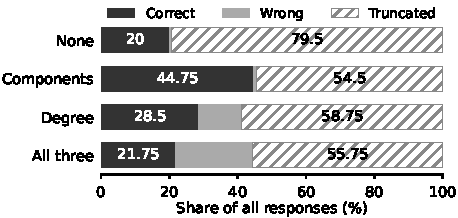
\includegraphics[width=\columnwidth]{edge_count_outcomes.pdf}
\caption{Qwen3-4B thinking on edge count: shares of \emph{all} responses. Conditions from top: none, component count, degree, all three node features. The bundle reduces truncation but raises wrong responses.} % [edgecount]
\label{fig:outcomes}
\end{figure}

\subsection{Model capacity and relational consistency}
The model arms differ in headroom. On unflagged cells, median no-primer correct shares are $66.0\%$ for plain 1.7B and $97.5\%$ for thinking 4B; % [arms]
the latter changes by at most $2.5$ points % [null4bt]
under any primer on degree, edge existence, or neighbor-set queries. Near-ceiling cells leave little room for gains, while edge count remains difficult under output limits. Plain 1.7B repeatedly outputs the maximum possible degree even when the primer states another value; thinking 1.7B retains an enumeration-based check and improves most where its baseline is weak. Averaging across arms would conceal this reversal.

The tasks permit a stricter check: a node's degree must equal the size of its returned neighbor set. For plain 4B, the share on which \emph{both} answers are correct falls from $85.75\%$ without a primer to $76.50\%$ with degree ($-9.2$ points, $q=.00032$), % [joint]
even though degree raises edge-count accuracy. The primer thus improves a graph-level sum while reducing cross-task correctness on the queried node. Conversely, the component-count diagnostic raises joint correctness to $95.00\%$ % [joint]
for the same arm, despite conveying no queried neighbor list. Joint accuracy is not a causal process test, but tests relational consistency more strictly than each task score alone.

\section{Discussion}
The strongest positive results establish that the model can sometimes use a statistic that directly contains the answer; they do not establish improved relational inference. This is inference-time answer disclosure, not evidence of training-set contamination: in the saved prompts, the degree sentence exactly states the queried degree in all $700/700$ checked cases, and half the listed degree sum equals the edge count in all $400/400$ checked cases. % [leak]
The handshaking identity makes degree's edge-count gain especially easy to misinterpret. The modest answer-free clustering effect in plain 1.7B replicates on fresh graphs despite selection from a broad screen; its early-node concentration and fewer missed neighbors suggest a change in graph-text reading. Response labels do not identify an internal attention mechanism.

The same score change carries different evidence across tasks. Degree gains on degree and edge count can be produced from the primer alone; clustering does not directly state the queried degree. Yet the clustering--filler comparison does not fully match wording or node location, and the effect is concentrated on early-listed nodes. Likewise, component count raises neighbor-set F1 even where its value is nearly constant. These controls narrow the explanations for each gain, but replication of a score difference does not verify the proposed reading procedure.

Two properties may help explain the selective results. First, printed RWSE values lose resolution in dense graphs: at $p=.50$ their two-decimal $(r^{(2)},r^{(3)})$ pairs form on average only $3.30$ distinct classes per graph, versus $12.50$ distinct stated degree values; % [rwse]
they are poorly suited to identifying a queried node's exact degree. Second, adding facts can displace a successful procedure: when plain 4B stops enumerating and instead retrieves a line of degree text, copying errors may exceed its baseline counting errors. Neither interpretation requires assuming the model has learned a graph invariant from text.

Pairing controls graph difficulty, but not constant-answer tasks, stochastic generation, node position or unequal dense-extension budgets. The study covers one model family, synthetic graphs, one encoding, rounded features and one phrasing. Description-order effects \citep{ge2025graph} reinforce the positional caveat; response labels do not identify an internal mechanism.

\paragraph{Future work.} Randomize node labels and primer position, match lengths and budgets, and test graph families with both cycle labels. Joint queries could test $d_v=|N(v)|$ and $2|E|=\sum_vd_v$.

\section{Conclusion}
Structural statistics can raise correct share; degree often supplies the answer outright, while other features have smaller, variable effects. Thinking can help yet increase truncation. Primer-only shortcuts, task-specific metrics, and all-response scoring are necessary to interpret graph reasoning gains.

\clearpage
\bibliography{custom}
\bibliographystyle{acl_natbib}
\clearpage
\appendix
\makeatletter
\setlength{\@fptop}{0pt}
\makeatother
\section{Evaluation Grid and Audit Trail}
\label{app:audit}

\paragraph{Coverage.} Every result in the body uses an undirected graph with exactly 40 nodes. % [setup]
The main sweep uses four graph densities for each task; only degree and edge existence additionally use three denser levels. Each model arm sees the same graph instances and seven conditions, so the paired key is (task, instance, model arm, condition). Table~\ref{tab:grid} makes the task-specific coverage and scoring distinction explicit. A fixed-size node count and the observed all-positive cycle labels mean that those two tasks test prompt behavior rather than sensitivity to the graph.

\begin{table}[h]
\centering\footnotesize
\setlength{\tabcolsep}{4pt}
\begin{tabular}{lll}
\toprule
Question & Densities & Reported score\\
\midrule
Node degree & main + dense & Integer exact match\\
Connected nodes & main & Set-F1; exact set also\\
Edge count & main & Integer exact match\\
Node count & main & Integer exact match\\
Cycle check & main & Boolean exact match\\
Edge existence & main + dense & Raw, balanced, yes-rate\\
\bottomrule
\end{tabular}
\caption{Task coverage. ``Main'' denotes $p\in\{.10,.20,.35,.50\}$; ``dense'' denotes $p\in\{.65,.75,.85\}$. % [setup]
The yes-rate is calculated among finished responses.}
\label{tab:grid}
\end{table}

\paragraph{Primer audit.} Table~\ref{tab:primerlength} gives average preamble length in \emph{characters}. Component count and filler are diagnostics outside the three-feature bundle. Filler names nodes without stating structure; it is approximately length-matched to clustering but differs in wording. Degree states the queried value and, by summation, edge count. A blind solver that reads only primer text identifies this answer disclosure.

\begin{table}[h]
\centering\footnotesize
\setlength{\tabcolsep}{4pt}
\begin{tabular}{lrp{3.1cm}}
\toprule
Condition & Mean chars & Information\\
\midrule
Components & 37 & Number of connected components\\ % [length]
Degree & 891 & Degree for each node\\ % [length]
Clustering & 1,629 & Local clustering for each node\\ % [length]
RWSE & 2,949 & Two rounded return values per node\\ % [length]
All three & 4,691 & Degree, clustering and RWSE\\ % [length]
Filler & 1,829 & Node names, no graph statistic\\ % [length]
\bottomrule
\end{tabular}
\caption{Mean preamble length in characters, not model tokens, over the main-sweep graphs. The no-primer control adds no preamble.} % [length]
\label{tab:primerlength}
\end{table}

\paragraph{Edge-existence diagnostic.} Table~\ref{tab:edgeprofile} compares the same prompts within each dense level. These descriptive figures make the class-balance and decision-bias argument checkable: raw accuracy, balanced accuracy and yes-rate must be read together, since the proportion of actual edges changes with density.

\begin{table}[h]
\centering\footnotesize
\setlength{\tabcolsep}{4pt}
\begin{tabular}{llrrr}
\toprule
$p$ & Primer & Raw acc. & Bal. acc. & Yes-rate\\
\midrule
.65 & none & .680 & .529 & .980\\ % [metric-audit-edge]
.65 & all & .760 & .647 & .900\\ % [metric-audit-edge]
.75 & none & .770 & .521 & .990\\ % [metric-audit-edge]
.75 & all & .860 & .723 & .880\\ % [metric-audit-edge]
.85 & none & .860 & .533 & .990\\ % [metric-audit-edge]
.85 & all & .890 & .661 & .940\\ % [metric-audit-edge]
\bottomrule
\end{tabular}
\caption{Plain Qwen3-1.7B on edge existence at high density. Raw and balanced accuracy use every prompt; yes-rate uses finished answers. These cells have no truncation. Values are descriptive, without a per-density BH claim.}
\label{tab:edgeprofile}
\end{table}

\paragraph{Scoring and provenance.} A generation that reaches its output cap is \emph{truncated}, even if text before the cap resembles an answer. The three outcome shares have the same denominator: every graph prompt in that condition. Set-F1 likewise uses all prompts and scores a truncated response as zero; yes-rate alone is conditional on finishing. Exact McNemar tests compare paired correctness, with Benjamini--Hochberg $q$-values within each (arm, task, control) family. For the supplemental F1 analysis, we pair graph instances, use random-sign tests of the mean F1 difference and adjust the six primer contrasts within each arm; bootstrap intervals resample pairs. Only $q<.05$ is treated as significant. Cells with at least 15\% truncation on either side are flagged and omitted from pooled low-truncation summaries, not from their own displayed results. % [setup]

Tagged results come from GraphTalk's \texttt{results-sot}, commit \texttt{292046f} \citep{graphtalkresults2026}: \path{docs/results/n40-sweep.md} and \path{csv2/raw-trends/primer_findings.txt}. \path{scripts/build_raw_frame.py} verifies saved gold labels; \path{scripts/primer_findings.py} rebuilds the tagged contrasts. Figure~\ref{fig:outcomes} uses \texttt{[edgecount]}; the bundled \path{metric_audit.py} and \path{primary_metric_tables.py} regenerate the primary-metric appendix from recorded responses.

\begin{table*}[t]
\centering\scriptsize
\setlength{\tabcolsep}{3.4pt}
\begin{tabular}{llrrrrrrr}
\toprule
Task & Arm & None & Degree & Cluster. & RWSE & All & Comp. & Filler\\
\midrule
Degree & 1.7P & 60.50 & $+7.5^{*}$ & $+3.0$ & $+4.0$ & $+10.2^{*}$ & $+1.8$ & $-0.5$\\ % [main]
 & 1.7T & 76.25 & $+8.8^{*}$ & $+1.5$ & $+2.5$ & $+12.2^{*}$ & $-1.0$ & $-3.0$\\ % [main]
 & 4P & 99.25 & $-6.5^{*}$ & $-0.5$ & $-2.2^{*}$ & $-8.0^{*}$ & $+0.2$ & $-0.5$\\ % [main]
 & 4T & 97.00 & $+2.5$ & $+1.8$ & $-1.2$ & $+0.5$ & $+0.2$ & $+2.0$\\ % [main]
\addlinespace[2pt]
Neighbors & 1.7P & 72.50 & $+3.5$ & $+1.2$ & $+1.0$ & $+2.0$ & $+0.8$ & $-6.2^{*}$\\ % [main]
 & 1.7T & 78.75 & $+6.2^{*}$ & $+2.0$ & $+0.2$ & $+6.2^{*}$ & $+2.5$ & $+2.5$\\ % [main]
 & 4P & 86.00 & $-3.0$ & $+1.0$ & $+0.0$ & $-2.8$ & $+9.2^{*}$ & $-12.5^{*}$\\ % [main]
 & 4T & 95.50 & $+0.5$ & $-0.8$ & $+0.5$ & $-1.2$ & $+0.5$ & $+1.2$\\ % [main]
\addlinespace[2pt]
Edge count & 1.7P & 1.25 & $+3.0^{\dagger}$ & $-0.5^{\dagger}$ & $-0.8^{\dagger}$ & $+0.8^{\dagger}$ & $-1.0^{\dagger}$ & $-0.5^{\dagger}$\\ % [main]
 & 1.7T & 15.75 & $-3.2^{\dagger}$ & $-1.3^{\dagger}$ & $-3.2^{\dagger}$ & $+5.0^{\dagger}$ & $-0.8^{\dagger}$ & $-1.5^{\dagger}$\\ % [main]
 & 4P & 2.00 & $+27.2^{*}$ & $-1.2$ & $-1.5$ & $+3.8^{*}$ & $-1.2$ & $+1.2$\\ % [main]
 & 4T & 20.00 & $+8.5^{*\dagger}$ & $+24.8^{*\dagger}$ & $+10.2^{*\dagger}$ & $+1.8^{\dagger}$ & $+24.8^{*\dagger}$ & $+12.2^{*\dagger}$\\ % [main]
\addlinespace[2pt]
Edge exists & 1.7P & 70.50 & $+4.0$ & $+3.8$ & $+5.0$ & $+11.5^{*}$ & $-8.2^{*}$ & $-15.8^{*}$\\ % [main]
 & 1.7T & 99.00 & $-2.5$ & $-1.0$ & $-1.2$ & $-1.8$ & $-0.8$ & $-0.5$\\ % [main]
 & 4P & 90.50 & $-4.8^{*}$ & $+4.0^{*}$ & $-10.0^{*}$ & $-10.0^{*}$ & $-2.8$ & $-7.0^{*}$\\ % [main]
 & 4T & 99.75 & $+0.0$ & $-0.8$ & $-1.2$ & $-1.0$ & $-0.5$ & $+0.0$\\ % [main]
\midrule
Node count & 1.7P & 31.50 & $+6.8^{*}$ & $+67.2^{*}$ & $+2.0$ & $+47.0^{*}$ & $+21.2^{*}$ & $+39.8^{*}$\\ % [main]
 & 1.7T & 91.00 & $+5.5^{*}$ & $+9.0^{*}$ & $+9.0^{*}$ & $+9.0^{*}$ & $+1.5$ & $+9.0^{*}$\\ % [main]
 & 4P & 90.25 & $+8.0^{*}$ & $+8.8^{*}$ & $+9.2^{*}$ & $+9.8^{*}$ & $+9.0^{*}$ & $+9.2^{*}$\\ % [main]
 & 4T & 99.50 & $+0.2$ & $+0.2$ & $+0.2$ & $+0.5$ & $+0.0$ & $+0.5$\\ % [main]
\addlinespace[2pt]
Cycle & 1.7P & 90.75 & $-17.5^{*\dagger}$ & $+8.5^{*}$ & $-0.2$ & $+7.0^{*}$ & $+2.0$ & $+3.0$\\ % [main]
 & 1.7T & 97.00 & $-21.8^{*\dagger}$ & $-0.5$ & $+2.2^{*}$ & $-0.8$ & $-7.5^{*}$ & $+3.0^{*}$\\ % [main]
 & 4P & 99.00 & $-2.2$ & $+0.5$ & $-0.2$ & $-0.2$ & $-2.0$ & $-0.5$\\ % [main]
 & 4T & 99.25 & $-5.5^{*}$ & $+0.0$ & $+0.2$ & $-0.5$ & $-3.2^{*}$ & $+0.5$\\ % [main]
\bottomrule
\end{tabular}
\caption{Complete main-sweep correct shares: no-primer baseline (percent of all prompts) and paired primer changes (points) on the same $40$-node graphs at $p\leq .50$. P/T: plain/thinking. $^{*}$ denotes $q<.05$ within the (arm, task, control) family; $^{\dagger}$ flags at least $15\%$ truncation on either side. For neighbor sets, this is exact-set correctness; primary Set-F1 is in Table~\ref{tab:f1}. Node count and cycle have constant gold labels. Values are rounded from the tagged [main] results.} % [setup] [main]
\label{tab:matrix}
\end{table*}

\begin{table*}[t]
\centering
\begin{minipage}[t]{.48\textwidth}
\centering\footnotesize\setlength{\tabcolsep}{2.1pt}
\textbf{(a) Neighbor-set Set-F1}\par\smallskip
\begin{tabular}{llrrr}
\toprule
Arm & Primer & None & With & $\Delta$; $q$\\
\midrule
1.7P & filler & 0.9721 & 0.9624 & $-0.0096$; 0.3114\\ % [metric-audit-f1]
1.7P & components & 0.9721 & 0.9716 & $-0.0004$; 0.9503\\ % [metric-audit-f1]
1.7P & clustering & 0.9721 & 0.9724 & $+0.0003$; 0.9503\\ % [metric-audit-f1]
1.7P & rwse & 0.9721 & 0.9702 & $-0.0018$; 0.9503\\ % [metric-audit-f1]
1.7P & degree & 0.9721 & 0.9794 & $+0.0074$; 0.3352\\ % [metric-audit-f1]
1.7P & all & 0.9721 & 0.9626 & $-0.0094$; 0.3846\\ % [metric-audit-f1]
\addlinespace[2pt]
1.7T & filler & 0.9732 & 0.9769 & $+0.0037$; 0.8851\\ % [metric-audit-f1]
1.7T & components & 0.9732 & 0.9726 & $-0.0006$; 0.9942\\ % [metric-audit-f1]
1.7T & clustering & 0.9732 & 0.9830 & $+0.0098$; 0.4254\\ % [metric-audit-f1]
1.7T & rwse & 0.9732 & 0.9577 & $-0.0156$; 0.4254\\ % [metric-audit-f1]
1.7T & degree & 0.9732 & 0.9627 & $-0.0105$; 0.4254\\ % [metric-audit-f1]
1.7T & all & 0.9732 & 0.9733 & $+0.0001$; 0.9942\\ % [metric-audit-f1]
\addlinespace[2pt]
4P & filler & 0.9871 & 0.9660 & $-0.0212$; 0.0001\\ % [metric-audit-f1]
4P & components & 0.9871 & 0.9976 & $+0.0105$; 0.0001\\ % [metric-audit-f1]
4P & clustering & 0.9871 & 0.9845 & $-0.0026$; 0.5411\\ % [metric-audit-f1]
4P & rwse & 0.9871 & 0.9776 & $-0.0095$; 0.0681\\ % [metric-audit-f1]
4P & degree & 0.9871 & 0.9768 & $-0.0103$; 0.0379\\ % [metric-audit-f1]
4P & all & 0.9871 & 0.9743 & $-0.0128$; 0.0209\\ % [metric-audit-f1]
\addlinespace[2pt]
4T & filler & 0.9636 & 0.9720 & $+0.0084$; 0.8279\\ % [metric-audit-f1]
4T & components & 0.9636 & 0.9641 & $+0.0006$; 0.8956\\ % [metric-audit-f1]
4T & clustering & 0.9636 & 0.9544 & $-0.0092$; 0.8279\\ % [metric-audit-f1]
4T & rwse & 0.9636 & 0.9676 & $+0.0041$; 0.8279\\ % [metric-audit-f1]
4T & degree & 0.9636 & 0.9685 & $+0.0050$; 0.8279\\ % [metric-audit-f1]
4T & all & 0.9636 & 0.9551 & $-0.0084$; 0.8279\\ % [metric-audit-f1]
\bottomrule
\end{tabular}
\end{minipage}\hfill
\begin{minipage}[t]{.48\textwidth}
\centering\footnotesize\setlength{\tabcolsep}{2.0pt}
\textbf{(b) Edge-existence decisions}\par\smallskip
\begin{tabular}{llrrrr}
\toprule
Arm & Primer & Raw & Bal. & Yes & Trunc.\\
\midrule
1.7P & none & 0.705 & 0.799 & 0.562 & 0.000\\ % [metric-audit-edge-main]
1.7P & degree & 0.745 & 0.823 & 0.517 & 0.000\\ % [metric-audit-edge-main]
1.7P & clustering & 0.743 & 0.824 & 0.525 & 0.000\\ % [metric-audit-edge-main]
1.7P & rwse & 0.755 & 0.827 & 0.501 & 0.003\\ % [metric-audit-edge-main]
1.7P & all & 0.820 & 0.877 & 0.448 & 0.000\\ % [metric-audit-edge-main]
\addlinespace[2pt]
1.7T & none & 0.990 & 0.990 & 0.271 & 0.003\\ % [metric-audit-edge-main]
1.7T & degree & 0.965 & 0.976 & 0.299 & 0.005\\ % [metric-audit-edge-main]
1.7T & clustering & 0.980 & 0.986 & 0.286 & 0.003\\ % [metric-audit-edge-main]
1.7T & rwse & 0.978 & 0.982 & 0.283 & 0.003\\ % [metric-audit-edge-main]
1.7T & all & 0.973 & 0.981 & 0.295 & 0.000\\ % [metric-audit-edge-main]
\addlinespace[2pt]
4P & none & 0.905 & 0.932 & 0.357 & 0.000\\ % [metric-audit-edge-main]
4P & degree & 0.858 & 0.903 & 0.407 & 0.005\\ % [metric-audit-edge-main]
4P & clustering & 0.945 & 0.963 & 0.323 & 0.000\\ % [metric-audit-edge-main]
4P & rwse & 0.805 & 0.867 & 0.463 & 0.000\\ % [metric-audit-edge-main]
4P & all & 0.805 & 0.867 & 0.461 & 0.003\\ % [metric-audit-edge-main]
\addlinespace[2pt]
4T & none & 0.998 & 0.998 & 0.268 & 0.003\\ % [metric-audit-edge-main]
4T & degree & 0.998 & 0.998 & 0.268 & 0.003\\ % [metric-audit-edge-main]
4T & clustering & 0.990 & 0.993 & 0.270 & 0.010\\ % [metric-audit-edge-main]
4T & rwse & 0.985 & 0.987 & 0.269 & 0.015\\ % [metric-audit-edge-main]
4T & all & 0.988 & 0.992 & 0.271 & 0.013\\ % [metric-audit-edge-main]
\bottomrule
\end{tabular}
\end{minipage}
\caption{Primary-metric audit on the same $400$ main-sweep prompts per arm and condition. (a) Neighbor-set Set-F1, with truncations scored zero: each row gives the no-primer baseline, the primer score and paired difference; $q$ adjusts six contrasts per arm. Components and filler are diagnostics. (b) Edge-existence raw and balanced accuracy (Bal.) and truncation (Trunc.) use all prompts; yes-rate (Yes) uses finished answers. Compare each primer row with its arm's none row. Only raw-accuracy contrasts have BH tests in Table~\ref{tab:matrix}; other edge measures are descriptive. P/T: plain/thinking.} % [metric-audit-f1] [metric-audit-edge-main]
\label{tab:primarymetrics}
\end{table*}

\clearpage
\raggedbottom
\section{Screening and Focused Robustness Checks}
\label{app:pilot}
\label{app:robust}

\paragraph{Earlier screens.} The repository's \path{docs/results/README.md} indexes Gemma 4 E4B/12B and Qwen3-8B/14B, each in plain and thinking mode, on published $5$--$19$-node GraphQA graphs; it reports near-ceiling unprimed performance on most piloted tasks. % [docs/results/README.md]
A separate no-primer $20/40/80$-node screen has saved runs but \emph{unverified} older analysis. % [docs/results/README.md]
It documents the selection effort without proving any size or model optimal; the final paired study uses only Qwen3-1.7B/4B and $40$-node graphs. % [setup]

\paragraph{Selection and replication.} The clustering-on-degree condition emerged from a $40$-cell screen: $700$ dedicated graphs overlap it, while $2{,}100$ do not. % [rqselection]
The independent fresh seed gives $+4.2$ points ($p=.00055$), with screen-wide Bonferroni-adjusted $p=.022$; % [ddrep] [rqselection]
the dedicated contrasts have separately reported BH $q$-values. Overlap limits the independence of the larger dedicated run.

\paragraph{Sensitivity.} Split-half intermediate-headroom means remain $+13.9$ and $+16.2$ points for answer-carrying cells; % [splithalf]
they pool heterogeneous tasks and arms. The repository's \texttt{[bandsens]} checks truncation thresholds. Early IDs are also short, confounding position with tokenization. % [position]

\paragraph{Reproduction.} \path{robustness_audit.py} regenerates the tagged tests from saved responses; \path{robustness_audit.txt} contains their output. Screening and position use the repository's tagged reports. No new model inference was performed.

\paragraph{Fixed-size effect heterogeneity.} Table~\ref{tab:interactions} compares within-graph primer effects between density groups, including truncations as noncorrect outcomes. Welch tests compare graph-level differences, density-stratified bootstrap supplies intervals, and BH adjusts the three exploratory interactions. Different graphs populate each density, so the test does not isolate its causal role.

\begin{table}[t]
\centering\footnotesize
\setlength{\tabcolsep}{2.4pt}
\begin{tabular}{lrrrr}
\toprule
Arm / primer & Low & High & High--low & $q$\\
\midrule
1.7P / cluster. & $+3.81$ & $-0.67$ & $-4.48$ & $.00445$\\ % [interaction]
1.7T / cluster. & $+2.50$ & $-5.42$ & $-7.92$ & $<.001$\\ % [interaction]
1.7T / degree & $+11.31$ & $+24.75$ & $+13.44$ & $<.001$\\ % [interaction]
\bottomrule
\end{tabular}
\caption{Primer effects on degree correct share (points), each relative to no primer. Low: $p\leq .50$ ($1{,}600$ pairs); high: $p\geq .65$ ($1{,}200$ pairs). % [interaction]
High-minus-low graph-bootstrap intervals are $[-7.62,-1.42]$, $[-11.75,-4.04]$, and $[+9.12,+17.71]$ points in row order. % [interaction]
These three post hoc tests constitute the BH family.}
\label{tab:interactions}
\end{table}

\paragraph{Direct bundle contrast.} Across $300$ paired dense plain-4B degree queries, clustering alone is correct on $66.33\%$ versus $33.67\%$ with \emph{all} ($-32.67$ points, $95\%$ bootstrap interval $[-39.33,-25.67]$, $q<.001$ across six alternatives). % [bundle-direct]
Neither condition truncates. All six paired comparisons appear in \path{robustness_audit.txt}. Length and order remain confounded.

\end{document}
